\chapter{Markov Chain}

\begin{notation}
	Let $(X_n)_{n\geq0}$ be a Markov chain on the state space $S$, $x\in S$, and let $E$ be an event. Then
	\[  \prob_x(E) = \prob(E|X_0=x) . \]
\end{notation}


\begin{example}
	It is a good practice to derive the value of the transition probability of a simple Markov chain using the first principles. Consider the Markov chain representing a lamp that turns on with probability $1/2$ and turns off with probability $1/2$, and stays at the old state with probability $1/2$. Thus we will have the following diagram for this Markov chain.
	\begin{figure}[h!]
	\centering
	
	


\tikzset{every picture/.style={line width=0.75pt}} %set default line width to 0.75pt        

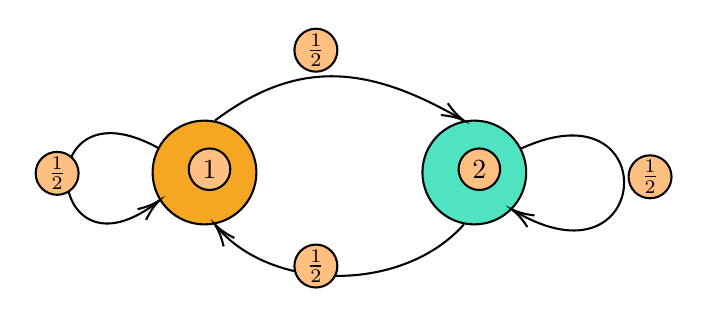
\begin{tikzpicture}[x=0.75pt,y=0.75pt,yscale=-1,xscale=1]
	%uncomment if require: \path (0,300); %set diagram left start at 0, and has height of 300
	
	%Shape: Circle [id:dp10052394937221254] 
	\draw  [fill={rgb, 255:red, 245; green, 166; blue, 35 }  ,fill opacity=1 ] (110,105) .. controls (110,91.19) and (121.19,80) .. (135,80) .. controls (148.81,80) and (160,91.19) .. (160,105) .. controls (160,118.81) and (148.81,130) .. (135,130) .. controls (121.19,130) and (110,118.81) .. (110,105) -- cycle ;
	%Shape: Circle [id:dp9437193586251307] 
	\draw  [fill={rgb, 255:red, 80; green, 227; blue, 194 }  ,fill opacity=1 ] (240,105) .. controls (240,91.19) and (251.19,80) .. (265,80) .. controls (278.81,80) and (290,91.19) .. (290,105) .. controls (290,118.81) and (278.81,130) .. (265,130) .. controls (251.19,130) and (240,118.81) .. (240,105) -- cycle ;
	%Curve Lines [id:da17352138739767575] 
	\draw    (140,80) .. controls (179.6,50.3) and (213.32,53.02) .. (258.62,79.2) ;
	\draw [shift={(260,80)}, rotate = 210.34] [color={rgb, 255:red, 0; green, 0; blue, 0 }  ][line width=0.75]    (10.93,-3.29) .. controls (6.95,-1.4) and (3.31,-0.3) .. (0,0) .. controls (3.31,0.3) and (6.95,1.4) .. (10.93,3.29)   ;
	%Curve Lines [id:da2659131152083798] 
	\draw    (141.59,131.91) .. controls (168.23,162.45) and (230.6,163.07) .. (260,130) ;
	\draw [shift={(140,130)}, rotate = 51.62] [color={rgb, 255:red, 0; green, 0; blue, 0 }  ][line width=0.75]    (10.93,-3.29) .. controls (6.95,-1.4) and (3.31,-0.3) .. (0,0) .. controls (3.31,0.3) and (6.95,1.4) .. (10.93,3.29)   ;
	%Curve Lines [id:da5459168562000609] 
	\draw    (113,93.33) .. controls (50.31,58.59) and (57.92,161.7) .. (112.51,119.07) ;
	\draw [shift={(113.33,118.41)}, rotate = 141.3] [color={rgb, 255:red, 0; green, 0; blue, 0 }  ][line width=0.75]    (10.93,-3.29) .. controls (6.95,-1.4) and (3.31,-0.3) .. (0,0) .. controls (3.31,0.3) and (6.95,1.4) .. (10.93,3.29)   ;
	%Curve Lines [id:da26931738393220694] 
	\draw    (287.67,93.41) .. controls (356.99,61.57) and (351.39,163.71) .. (284.02,123.36) ;
	\draw [shift={(283,122.74)}, rotate = 31.58] [color={rgb, 255:red, 0; green, 0; blue, 0 }  ][line width=0.75]    (10.93,-3.29) .. controls (6.95,-1.4) and (3.31,-0.3) .. (0,0) .. controls (3.31,0.3) and (6.95,1.4) .. (10.93,3.29)   ;
	
	% Text Node
	\draw (130,96) node [anchor=north west][inner sep=0.75pt]   [align=left] {1};
	% Text Node
	\draw (260,96) node [anchor=north west][inner sep=0.75pt]   [align=left] {2};
	% Text Node
	\draw (56.33,97.73) node [anchor=north west][inner sep=0.75pt]   {$\frac{1}{2}$};
	% Text Node
	\draw (342,99.4) node [anchor=north west][inner sep=0.75pt]  {$\frac{1}{2}$};
	% Text Node
	\draw (181,38.4) node [anchor=north west][inner sep=0.75pt]  {$\frac{1}{2}$};
	% Text Node
	\draw (181,142.4) node [anchor=north west][inner sep=0.75pt]   {$\frac{1}{2}$};
	
	
\end{tikzpicture}
\end{figure}\\
	In this example, the state space is $S = \{0,1\}$, and the sample space is
	\[ \Omega = \{ (x_1,x_2,\cdots): x_i \in S \} \]
	which is basically the set of all sequences of one's and zero's. Given this, the random variables $(X_n)_n$ defined t be
	\[  X_n (\omega) = x_n, \]  
	where $\omega \in \Omega$ and $x_n$ is the $n$-th letter in $\omega$. Intuitively speaking, we know that 
	\[  P(1,0) = \prob(X_{n+1} = 1 | X_n = 0) = \frac{1}{2}. \]
	However, here we want to derive that number more explicitly by working directly with the elements of the probability space. First, we need to determine the event associated with $X_{n+1} = 1$. This is the event that has elements where the $n+1$-th position is 1. I.e.
	\[  E = \{  (x_1,x_2, \cdots, x_n, 1, x_{n+2}, \cdots) : x_i \in S\}.  \]
	Similarly, we have
	\[ F = \{ (x_1,x_2, \cdots, x_{n-1},0,x_{n+1},\cdots): x_i \in S \}. \]
	So we have
	\[ \prob(X_{n+1} = 1 | X_n = 0)  = \prob(E|F) = \frac{\prob(E\cap F)}{\prob(F)} =\frac{\prob(E\cap F)}{\prob(F\cap E) + \prob(F\cap E^c)} = \frac{\frac{1}{\abs{\Omega}}}{\frac{1}{\abs{\Omega}} + \frac{1}{\abs{\Omega}}} = \frac{1}{2}. \]
	Note that $\prob(E\cap F) = \frac{1}{\abs{\Omega}}$, since out of many combinations of the sequence of zeros and ones, there is one one sequence whose $n$-th place is 0 and $n+1$-th place is 1. Furthermore, $\prob(F\cap E^c) = \frac{1}{\abs{\Omega}}$ as there is only one string where its $n$-th and $(n+1)$-th string are both zero. 
\end{example}

\begin{example}[Gambler's Ruin]
	Suppose Alice and Bob have in total of $N$ coins. Alice and Bob play a game with a fair coin. When Alice wins, gets a coin from Bop, and vise versa. What is the probability that Alice wins if she starts with $0\leq a \leq N$ coins.
	
	\begin{solution}
		There are many ways to tackle a probability problem like this and the solution presented here is not the only way to find the solution to this problem. We want to model this with Markov chain whose state space is $\{0,1,2,\cdots,N\}$. Thus $X_n$ represents the fortune of Alice after playing the games for $n$ times. 
		\begin{figure}[h!]
	\centering
	
	
	
	\tikzset{every picture/.style={line width=0.75pt}} %set default line width to 0.75pt        
	
	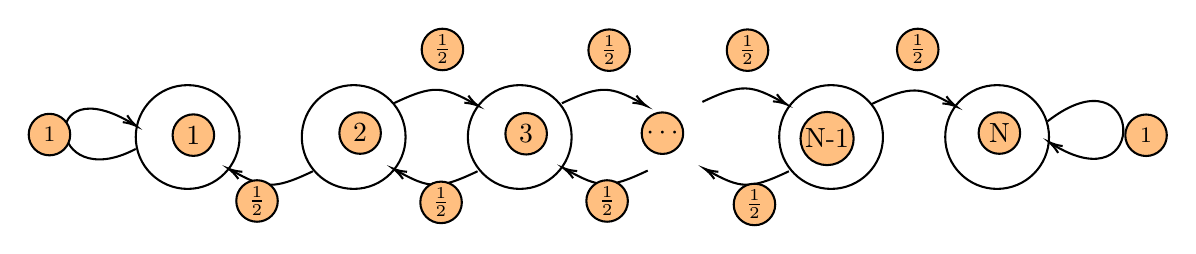
\begin{tikzpicture}[x=0.75pt,y=0.75pt,yscale=-1,xscale=1]
		%uncomment if require: \path (0,300); %set diagram left start at 0, and has height of 300
		
		%Shape: Circle [id:dp09774088338298847] 
		\draw   (100,125) .. controls (100,111.19) and (111.19,100) .. (125,100) .. controls (138.81,100) and (150,111.19) .. (150,125) .. controls (150,138.81) and (138.81,150) .. (125,150) .. controls (111.19,150) and (100,138.81) .. (100,125) -- cycle ;
		%Shape: Circle [id:dp43482816564378113] 
		\draw   (180,125) .. controls (180,111.19) and (191.19,100) .. (205,100) .. controls (218.81,100) and (230,111.19) .. (230,125) .. controls (230,138.81) and (218.81,150) .. (205,150) .. controls (191.19,150) and (180,138.81) .. (180,125) -- cycle ;
		%Shape: Circle [id:dp7628960050576648] 
		\draw   (260,125) .. controls (260,111.19) and (271.19,100) .. (285,100) .. controls (298.81,100) and (310,111.19) .. (310,125) .. controls (310,138.81) and (298.81,150) .. (285,150) .. controls (271.19,150) and (260,138.81) .. (260,125) -- cycle ;
		%Shape: Circle [id:dp3849023603262607] 
		\draw   (410,125) .. controls (410,111.19) and (421.19,100) .. (435,100) .. controls (448.81,100) and (460,111.19) .. (460,125) .. controls (460,138.81) and (448.81,150) .. (435,150) .. controls (421.19,150) and (410,138.81) .. (410,125) -- cycle ;
		%Shape: Circle [id:dp902561209940324] 
		\draw   (490,125) .. controls (490,111.19) and (501.19,100) .. (515,100) .. controls (528.81,100) and (540,111.19) .. (540,125) .. controls (540,138.81) and (528.81,150) .. (515,150) .. controls (501.19,150) and (490,138.81) .. (490,125) -- cycle ;
		%Curve Lines [id:da2277389625716164] 
		\draw    (224.33,108.74) .. controls (243.31,99.74) and (247.7,100.35) .. (263.26,109.02) ;
		\draw [shift={(265,110)}, rotate = 209.42] [color={rgb, 255:red, 0; green, 0; blue, 0 }  ][line width=0.75]    (6.56,-1.97) .. controls (4.17,-0.84) and (1.99,-0.18) .. (0,0) .. controls (1.99,0.18) and (4.17,0.84) .. (6.56,1.97)   ;
		%Curve Lines [id:da8597065575180056] 
		\draw    (305.33,108.74) .. controls (324.31,99.74) and (328.7,100.35) .. (344.26,109.02) ;
		\draw [shift={(346,110)}, rotate = 209.42] [color={rgb, 255:red, 0; green, 0; blue, 0 }  ][line width=0.75]    (6.56,-1.97) .. controls (4.17,-0.84) and (1.99,-0.18) .. (0,0) .. controls (1.99,0.18) and (4.17,0.84) .. (6.56,1.97)   ;
		%Curve Lines [id:da07306821532750352] 
		\draw    (454.67,109.08) .. controls (473.65,100.07) and (478.03,100.69) .. (493.59,109.36) ;
		\draw [shift={(495.33,110.33)}, rotate = 209.42] [color={rgb, 255:red, 0; green, 0; blue, 0 }  ][line width=0.75]    (6.56,-1.97) .. controls (4.17,-0.84) and (1.99,-0.18) .. (0,0) .. controls (1.99,0.18) and (4.17,0.84) .. (6.56,1.97)   ;
		%Shape: Boxed Bezier Curve [id:dp2584084656510479] 
		\draw    (185.33,141.51) .. controls (166.35,150.51) and (161.97,149.9) .. (146.41,141.23) ;
		\draw [shift={(144.67,140.25)}, rotate = 29.42] [color={rgb, 255:red, 0; green, 0; blue, 0 }  ][line width=0.75]    (6.56,-1.97) .. controls (4.17,-0.84) and (1.99,-0.18) .. (0,0) .. controls (1.99,0.18) and (4.17,0.84) .. (6.56,1.97)   ;
		%Shape: Boxed Bezier Curve [id:dp08231579755337615] 
		\draw    (264.67,141.51) .. controls (245.69,150.51) and (241.3,149.9) .. (225.74,141.23) ;
		\draw [shift={(224,140.25)}, rotate = 29.42] [color={rgb, 255:red, 0; green, 0; blue, 0 }  ][line width=0.75]    (6.56,-1.97) .. controls (4.17,-0.84) and (1.99,-0.18) .. (0,0) .. controls (1.99,0.18) and (4.17,0.84) .. (6.56,1.97)   ;
		%Shape: Boxed Bezier Curve [id:dp9912054198682547] 
		\draw    (346.67,141.17) .. controls (327.69,150.18) and (323.3,149.56) .. (307.74,140.89) ;
		\draw [shift={(306,139.92)}, rotate = 29.42] [color={rgb, 255:red, 0; green, 0; blue, 0 }  ][line width=0.75]    (6.56,-1.97) .. controls (4.17,-0.84) and (1.99,-0.18) .. (0,0) .. controls (1.99,0.18) and (4.17,0.84) .. (6.56,1.97)   ;
		%Shape: Boxed Bezier Curve [id:dp49752798194307046] 
		\draw    (414.67,141.51) .. controls (395.69,150.51) and (391.3,149.9) .. (375.74,141.23) ;
		\draw [shift={(374,140.25)}, rotate = 29.42] [color={rgb, 255:red, 0; green, 0; blue, 0 }  ][line width=0.75]    (6.56,-1.97) .. controls (4.17,-0.84) and (1.99,-0.18) .. (0,0) .. controls (1.99,0.18) and (4.17,0.84) .. (6.56,1.97)   ;
		%Curve Lines [id:da6769266285825299] 
		\draw    (373,108.08) .. controls (391.98,99.07) and (396.37,99.69) .. (411.93,108.36) ;
		\draw [shift={(413.67,109.33)}, rotate = 209.42] [color={rgb, 255:red, 0; green, 0; blue, 0 }  ][line width=0.75]    (6.56,-1.97) .. controls (4.17,-0.84) and (1.99,-0.18) .. (0,0) .. controls (1.99,0.18) and (4.17,0.84) .. (6.56,1.97)   ;
		%Curve Lines [id:da5266663507857827] 
		\draw    (539.33,117.41) .. controls (585.53,81.44) and (589.59,158.51) .. (541.47,128.36) ;
		\draw [shift={(540,127.41)}, rotate = 33.33] [color={rgb, 255:red, 0; green, 0; blue, 0 }  ][line width=0.75]    (6.56,-1.97) .. controls (4.17,-0.84) and (1.99,-0.18) .. (0,0) .. controls (1.99,0.18) and (4.17,0.84) .. (6.56,1.97)   ;
		%Curve Lines [id:da13630212552736864] 
		\draw    (100,130.74) .. controls (56.77,153.51) and (52.74,90.36) .. (98.92,118.85) ;
		\draw [shift={(100.33,119.74)}, rotate = 212.76] [color={rgb, 255:red, 0; green, 0; blue, 0 }  ][line width=0.75]    (6.56,-1.97) .. controls (4.17,-0.84) and (1.99,-0.18) .. (0,0) .. controls (1.99,0.18) and (4.17,0.84) .. (6.56,1.97)   ;
		
		% Text Node
		\draw (120.33,116.67) node [anchor=north west][inner sep=0.75pt]   [align=left] {1};
		% Text Node
		\draw (200.67,115.67) node [anchor=north west][inner sep=0.75pt]   [align=left] {2};
		% Text Node
		\draw (280.67,116) node [anchor=north west][inner sep=0.75pt]   [align=left] {3};
		% Text Node
		\draw (423.67,116.33) node [anchor=north west][inner sep=0.75pt]   [align=left] {N-1};
		% Text Node
		\draw (508.67,115.67) node [anchor=north west][inner sep=0.75pt]   [align=left] {N};
		% Text Node
		\draw (151,148.4) node [anchor=north west][inner sep=0.75pt]  [font=\footnotesize]  {$\frac{1}{2}$};
		% Text Node
		\draw (239.67,149.07) node [anchor=north west][inner sep=0.75pt]  [font=\footnotesize]  {$\frac{1}{2}$};
		% Text Node
		\draw (319.67,148.4) node [anchor=north west][inner sep=0.75pt]  [font=\footnotesize]  {$\frac{1}{2}$};
		% Text Node
		\draw (390.67,150.07) node [anchor=north west][inner sep=0.75pt]  [font=\footnotesize]  {$\frac{1}{2}$};
		% Text Node
		\draw (469.33,75.4) node [anchor=north west][inner sep=0.75pt]  [font=\footnotesize]  {$\frac{1}{2}$};
		% Text Node
		\draw (387.33,75.73) node [anchor=north west][inner sep=0.75pt]  [font=\footnotesize]  {$\frac{1}{2}$};
		% Text Node
		\draw (320.67,75.73) node [anchor=north west][inner sep=0.75pt]  [font=\footnotesize]  {$\frac{1}{2}$};
		% Text Node
		\draw (240.33,75.4) node [anchor=north west][inner sep=0.75pt]  [font=\footnotesize]  {$\frac{1}{2}$};
		% Text Node
		\draw (579.33,116.73) node [anchor=north west][inner sep=0.75pt]  [font=\footnotesize]  {$1$};
		% Text Node
		\draw (51,116.4) node [anchor=north west][inner sep=0.75pt]  [font=\footnotesize]  {$1$};
		% Text Node
		\draw (346.33,115.73) node [anchor=north west][inner sep=0.75pt]    {$\cdots $};
		
		
	\end{tikzpicture}
\end{figure} \\
		Let $p_a$ be the probability of Alice wining if she starts with $a$ coins. First, observe that $p_0 = 0$ and $p_N= 1$. Let $E$ denote that event of Alice wining the whole game. Also, let $F_1$ be the event in which she looses the first game and $F_2$ the event in which she wins the first game. Then
		\[ p_a = \prob_a(E) =  \underbrace{\prob_a(E | F_1)}_{\prob(E|F_1,X_0=a)} \prob(F_1) + \underbrace{\prob_a(E|F_1^c)}_{\prob(E|F_1^c,X_0=a)}\prob(F_1^c) \]
		(note that this identity is actually true for any set $F_1$, but here $F_1$ is the specific event explained above). The probability that she looses or wins the first game is $\frac{1}{2}$. Also, observe that $\prob_a(E|F_1) = p_{a+1}$ (since if she wins the first game she will have one more coin) and $\prob_a(E|F_1^c) = p_{a-1}$. Thus 
		\[ p_a = \frac{1}{2}p_{a+1} + \frac{1}{2}p_{a-1}. \]
		Now we can solve this recurrent equation with the characterization polynomial which is $2 = X + 1/X$ or $X^2 - 2X + 1 = (X-1)^2 = 0$. Thus the characteristic polynomial has a double root. Thus 
		\[ p_a = (Aa + B)(1)^a = Aa + B. \]
		Since $p_0 = 0,\ p_N =1$, then it turns out that
		\[ p_a = \frac{a}{N}. \]
	\end{solution}
\end{example}

\begin{example}[Gambler's Ruin with Draw]
	Let Alice and Bob play Rock-Paper-Scissors. If Alice and Bob has a total of $N$ coins, and at each play, the winner gets one coin from the loser, what is the probability that Alice will win the game if he starts with $a$ coins. When they draw, then they repeat the game (or equivalently, they play another game without any coins exchange).
	
	\begin{solution}
		We need to do a first step analysis similar to what we did before. Let $E$ be the event that Alice wins the whole game, and the event $F=F_{-1}\cup F_0 \cup F_1$ where
		\begin{quote}
			$F_{-1}$: Alice loses the first game,\\
			$F_0$: Alice draws the first game,\\
			$F_1$: Alice wins the first game.
		\end{quote}
		It is clear that $\prob(F) = 1$, since the components are mutually disjoint. Thus $E\cap F_{-1},\ E\cap F_0,\ E\cap F_1$ are also mutually disjoints where. Thus we can write
		\[\prob_a(E) = \prob_a(E\cap F_{-1}) + \prob_a(E\cap F_0) + \prob_a(E\cap F_1)
				= \prob_a(E|F_{-1})\prob_a(F_{-1}) + \prob_a(E|F_0)\prob_a(F_0) + \prob_a(E|F_1)\prob_a(F_1).
		\]
		Since the game is fair we know
		\[ \prob_a(F_{-1}) = \prob_a(F_0) = \prob_a(F_1) = \frac{1}{3}.  \]
		Furthermore, we know
		\[ \prob_a(E|F_{-1}) = p_{a-1}, \qquad \prob_a(E|F_0) = p_a, \qquad \prob_a(E|F_1) = p_{a+1}. \]
		Thus the first step analysis will lead to the following identity.
		\[  \prob_a(E) = p_a = \frac{1}{3} ( p_{a-1} + p_{a} + p_{a+1}),\]
		which after simplification becomes
		\[ 2p_a = p_{a-1} + p_{a+1}, \]
		which is the same recursive formula we got in the previous example. So the possibility of the draw, will not change the behaviour of the system.
	\end{solution}
\end{example}


\begin{proposition}[First step argument]
	Let $(X_n)_{n\geq 0}$ be a Markov chain on the state space $S$. Let $x\in S$, and $W,Z \subset S$. Let $B$ be any event. Then
	\[ \prob_x(B) = \sum_{y:x\sim y} \prob_y(B)P(x,y). \]
	\label{prop:FirstTimeStepArgument}
\end{proposition}
\begin{proof}
	To prove the proposition above, we Let $E_i = \{ X_0=x, X_1=y_i \}$ where $y_i \sim x$. So, in words, we say that the event $E_i$ has occurred if $X_1 = y_i$. It is clear that $E_i \cap E_j = \emptyset$ where $i\neq j$. Thus $\bigcup_{i}(B\cap E_i) = B$. Thus 
	\[ \prob_x(B) = \sum_{i} \prob_x(B \cap E_i) = \sum_{i}\prob_x(B|E_i)\prob_x(E_i). \]
	In which $\prob_x(E_i) = \prob(E_i|X_0=x) = \prob(X_1=y_i|X_0=x) = P(x,y_i)  $. Also \[\prob_x(B|E_i) = \prob(B|X_1=y_i, X_0=x) = \prob(B|X_1=y_i) = \prob_{y_i}(B),\].
	in which we have used the Markov property. Thus we can write
	\[ P_x(B) = \sum_i \prob_{y_i}(B)P(x,y_i). \]
\end{proof}


\begin{example}
	Consider the a simple random walker on the following graph. Let $B = \{ T_{\tilde{x}} < T_{\set{\tilde{z},\tilde{y}}} \}$. Compute the probability $\prob_0(B)$.
	
	\begin{center}
		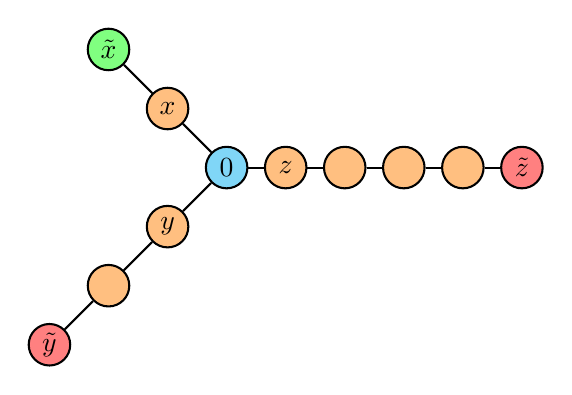
\begin{tikzpicture}[scale=1.5, every node/.style={circle, draw}]
			\tikzstyle{every node}=[circle, draw, fill=white,
			inner sep=0pt, minimum width=15pt]
			
			\node[fill=cyan!50] (a) at (0,0) {0};
			\node[fill=orange!50] (z1) at (1/2,0) {$z$};
			\node[fill=orange!50] (z2) at (2/2,0) {};
			\node[fill=orange!50] (z3) at (3/2,0) {\ };
			\node[fill=orange!50] (z4) at (4/2,0) {\ };
			\node[fill=red!50] (ze) at (5/2,0) {$\tilde{z}$};
			
			\node[fill=orange!50] (x1) at (-1/2,1/2) {$x$};
			\node[fill=green!50] (xe) at (-1,1) {$\tilde{x}$};
			
			\node[fill=orange!50] (y1) at (-1/2,-1/2) {$y$};
			\node[fill=orange!50] (y2) at (-2/2,-2/2) {};
			\node[fill=red!50] (ye) at (-3/2,-3/2) {$\tilde{y}$};
			
			
			\draw (a) -- (z1);
			\draw (z1) -- (z2);
			\draw (z2) -- (z3);
			\draw (z3) -- (z4);
			\draw (z4) -- (ze);
			
			\draw (a) -- (y1);
			\draw (y1) -- (y2);
			\draw (y2) -- (ye);
			
			\draw (a) -- (x1);
			\draw (x1) -- (xe);
			
		\end{tikzpicture}
	\end{center}
	
	\begin{solution}
		This problem is simply asking what is the probability that we hit $\tilde{x}$ state before hitting any of $\tilde{y}$ or $\tilde{z}$ states, given the fact that the random walker starts from the state $0$. To keep unnecessary details out of the way, we have only labeled the vertices that we will use in our analysis. We will have the following notation to simplify the solution
		\[ p_v = \prob_v(B), \]
		where $v$ is any vertex in the graph. Note that starting at 0, i.e. $X_0=0$, then going to any of the states $x,y$, or $z$, are mutually disjoint events, and the probability of the union of these events is one. With our first time step analysis (see \autoref{prop:FirstTimeStepArgument}) we can write
		\[ \prob_0(B) = \frac{1}{3} ( p_x + p_y + p_z). \]
		Now we need to analyze each of terms in the RHS. Let's start with $p_z$. Consider two events $\{ T_0 < T_{\tilde{z}}  \}$ and $\{ T_0 > T_{\tilde{z}}  \}$, where the first time is the event where the random walker hits the $0$ state before hitting the $\tilde{z}$ step first, and the second one is the vice versa. These two events are disjoint and the probability of the union is 1. Thus we write the conditional expansion of $p_z$ based on these events
		\[ p_z = \prob_z(B) = \prob_z(B|T_0 < T_{\tilde{z}})\prob_z(T_0 < T_{\tilde{z}}) + \prob_z(B|T_0 > T_{\tilde{z}})\prob_z(T_0 > T_{\tilde{z}}). \]
		We know that $\prob_z(B|T_0 > T_{\tilde{z}}) = \prob(B|X_0=z,X_i=\tilde{z})$ for some $i > 0$. From Markov property it follows that 
		\[ \prob(B|X_0=z,X_i=\tilde{z}) = \prob(B|X_i=\tilde{z}) = \prob(B|X_0 = \tilde{z})  = p_{\tilde{z}}.\]
		Also $\prob_z(B|T_0<T_{\tilde{z}}) = \prob_0(B) = p_0$ by the Markov property. Lastly, $\prob_z(T_0<T_{\tilde{z}})$ is determined by the Gambler's ruin method we say before, which is basically
		\[ \prob_z(T_0 < T_{\tilde{z}}) = \frac{5}{4}, \qquad \prob_z(T_0>T_{\tilde{z}}) = \frac{1}{5}. \]
		By doing the same kind of analysis for $p_x$ as well as $p_y$ we will get
		\[ p_z = \frac{4}{5}p_0 , \qquad p_y = \frac{2}{3}p_0, \qquad p_x =\frac{1}{2}p_0 + \frac{1}{2}. \]
		Now by substituting in the identity we got from the first time step argument, we can fine that 
		\[ p_0 = \frac{15}{31}, \]
		And this completes our solution for the problem.
	\end{solution}
	
\end{example}

\begin{example}
	Consider the graph $\gamma=  (V,E)$ drawn below. Set $Z = \{2,3\}$, and $W = \set{6,9}$. Compute $\prob_0(T_Z<T_W)$. In colors: we start at blue, win if we reach green, and lose of we reach red.
	
	\begin{center}
		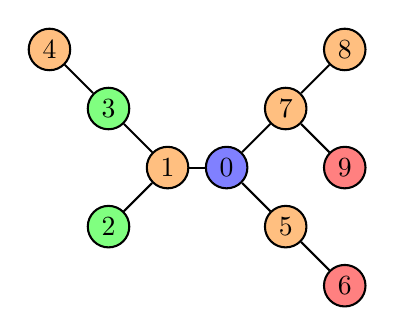
\begin{tikzpicture}[scale=1.5, every node/.style={circle, draw}]
			\tikzstyle{every node}=[circle, draw, fill=orange!50,
			inner sep=0pt, minimum width=15pt]
			
			\node[fill=blue!50] (n0) at (1/2,0) {0};
			\node (n1) at (0/2,0) {1};
			\node[fill=green!50] (n2) at (-1/2,-1/2) {2};
			\node[fill=green!50] (n3) at (-1/2,1/2) {3};
			\node (n4) at (-2/2,2/2) {4};
			\node (n5) at (2/2,-1/2) {5};
			\node[fill=red!50] (n6) at (3/2,-2/2) {6};
			\node (n7) at (2/2,1/2) {7};
			\node (n8) at (3/2,2/2) {8};
			\node[fill=red!50] (n9) at (3/2,0/2) {9};

			
			\draw (n0) -- (n1);
			\draw (n1) -- (n2);
			\draw (n1) -- (n3);
			\draw (n3) -- (n4);
			\draw (n0) -- (n7);
			\draw (n0) -- (n5);
			\draw (n5) -- (n6);
			\draw (n7) -- (n9);
			\draw (n7) -- (n8);
			
		\end{tikzpicture}
	\end{center}
\end{example}

\begin{solution}
	As always, we start with our powerful tool in hand, which is the first step argument (which is basically a special form of the more general conditional expansion). We start with first step argument at state $0$. We will get
	\[ \prob_0(B) = \frac{1}{3} (\prob_1(B) + \prob_7(B) + \prob_5(B) ), \]
	and now we need to analyze each of the terms in the right hand side. We start with $\prob_5(B)$ which is the most straight forward one. As we saw in the last example, we can analyze this state with a conditional expansion on the two disjoint events, whose union probability is 1. Let those two events be $\set{T_6 < T_0}$ (where the random walker hits the state $6$ before hitting the state $0$), and $\set{T_6 > T_0}$, where the random walker hits the state $0$ before hitting the state $6$. Thus the expansion will be
	\[ \prob_5(B) = \prob_5(B|T_6 < T_0) \prob_5(T_6 < T_0) + \prob_5(B|T_6 > T_0)\prob_5(T_6 > T_0). \]
	We know that if we hit the state $6$ before $0$, we have no chance to hit any of the green states (we will lose). Thus
	\[ \prob_5(B|T_6<T_0) = 0. \]
	And from the Gambler's ruin we know that $\prob_5(T_6>T_0) = 1/2$, and from the Markov property we know that $\prob_5(B|T_6>T_0) = \prob_0(B)$, because the conditional probability $\prob_5(B|T_6>T_0)$ is basically stating what is the probability of $B$ happening, if we start from $5$ and $X_i = 0$ for some $i$ in the future. Thus 
	\[ \prob_5(B) = \frac{\prob_0(B)}{2}. \]
	Now, we need to analyze the term $\prob_1(B)$. Again, at this step, we do another first step analysis.
	\[  \prob_1(B) = \frac{1}{3} (\underbrace{\prob_3(B)}_{=1} + \underbrace{\prob_2(B)}_{=1} +\prob_0(B)) = \frac{2+\prob_0(B)}{3}. \]
	Note that from the assumption, we know that if we reach any of green states, then we are declared winner, that is why we have $\prob_3(B) = \prob_2(B) = 1$. Now it only remains to analyze the term $\prob_7(B)$. Again, similar to the case above, we do a first time step argument
	\[ \prob_7(B) = \frac{1}{3} ( \prob_0(B) + \underbrace{\prob_8(B)}_{=\prob_7(B)} + \underbrace{\prob_9(B)}_{=0} ) \implies \prob_7(B) = \frac{\prob_0(B)}{2}.\]
	Note that $\prob_8(B) = \prob_7(B)$ by a first stem analysis when starting at the state $8$. Putting all of these terms back to the original identity we derived the first, we can conclude that 
	\[ p_0 = \prob_0(B) = \frac{2}{5}. \]
\end{solution}




\section{Solved Problems}
\begin{question} 
	If $A, B$ and $C$ are sets. prove the followings:
	\begin{enumerate}[(a)]
		\item $A \cap (B \cup C) = (A \cap B) \cup (A \cap C)$. \label{section-a}
		\item $C \textbackslash (A \cup B) = (C \textbackslash A) \cap (C \backslash B)$.
		
		\item $C \backslash (A \cap B) = (C \backslash A) \cup (C \backslash B) $.
		
	\end{enumerate}
	
	\begin{ans}
		\begin{enumerate}[(a)]
			\item 
			\begin{proof}
			Let $P, Q$, and $R$ be logical statements. We can show (using the truth table) that the following biconditional implication is a tautology. \[ P \wedge (Q \vee R) \Leftrightarrow (P \wedge Q) \vee (P \wedge R). \]
			Now let $x \in A \cap (B \cup C)$. Then $x \in A \wedge (x \in B \vee x \in C)$. Using the tautology above we can write $(x \in A \wedge x \in B) \vee (x \in A \wedge x \in C)$, thus $x \in (A \cap B) \cup (A \cap C) $, which means $A \cap (B \cap C) \subset (A \cap B) \cup (A \cap C)$. Conversely, let $x \in (A \cap B) \cup (A \cap C)$. By definition $(x \in A \wedge x \in B) \vee (x \in A \wedge x \in C)$. With the similar logic as above we can infer $(A \cap B) \cup (A \cap C) \subset A \cap (B \cup C)$. Thus $A \cap (B \cup C) = (A \cap B) \cup (A \cap C)$.
			\end{proof}
			
			\item 
			\begin{proof}
			Let $x \in C \backslash (A \cup B)$. By definition $x \in C \wedge x \notin (A \cup B) \biImp x \in C \wedge x \in \overline{A \cup B} \biImp x \in C \wedge x \in \bar{A} \cap \bar{B} \biImp x \in C \wedge (x \notin A \wedge x \notin B)$. Finally, using the following tautology 
			\[ P \wedge (Q \wedge R) \Leftrightarrow (P \wedge Q) \wedge (P \wedge R), \]
			we can write $(x \in C \wedge x \notin A) \wedge (x \in C \wedge x \notin B) \biImp x \in (C \backslash A) \cap (C \backslash B) $, thus $C \textbackslash (A \cup B) subset (C \textbackslash A) \cap (C \backslash B)$. The converse can be shown is true following the similar logic as below, thus inferring $C \textbackslash (A \cup B) = (C \textbackslash A) \cap (C \backslash B)$.
			\end{proof}
			
			\item \begin{proof}
			Let $x \in C \backslash (A \cap B)$. By definition $x \in C \wedge x \notin (A \cap B) \biImp x \in C \wedge x \in \overline{A \cap B} \biImp x \in C \wedge x \in \bar{A} \cup \bar{B} \biImp x \in C \wedge (x \notin A \vee x \notin B)$. Using the tautology in section (a),
			we can write $(x \in C \wedge x \notin A) \vee (x \in C \wedge x \notin B) \biImp x \in (C \backslash A) \cup (C \backslash B) $, thus $C \textbackslash (A \cap B) \subset (C \textbackslash A) \cup (C \backslash B)$. The converse can be shown is true following the similar logic as below, thus inferring $C \textbackslash (A \cap B) = (C \textbackslash A) \cup (C \backslash B)$.
			\end{proof}
			
			
			
			
		\end{enumerate}
	\end{ans}
\end{question}
\begin{problem}
	There are 6 coins on a table, each showing heads (H) or tails (T). In each step we 
	\begin{itemize}
		\item Select uniformly one of the coins. 
		\item If it is heads, toss it and replace on the table (with random side).
		\item If it sis tails, toss it. If it comes up heads, leave it at that. If it comes up tails, toss it a second time, and leave the result as it is.
		Let $X_n$ be the number of heads showing after $n$ such steps. Answer the following questions
		\begin{enumerate}[(a)]
			\item Determine the transition probabilities for this Markov chain.
			\item Draw the transition diagram and write the transition matrix.
			\item What is $\prob(X_2 = 4| X_0=5)$?
		\end{enumerate}
	\end{itemize}
\end{problem}
\begin{solution}
	\begin{enumerate}[(a)]
		\item To compute the transition probabilities, we need to perform the first step analysis. Let the events \[I = \set{X_1 = a+1},\qquad S = \set{X_1 = a},\qquad D = \set{X_1 = a-1},\]
		where $0 \leq a \leq 6$ is the number of heads. So to compute the transition probabilities, we need to compute
		\[ P(a,a+1) = \prob_a(I), \qquad P(a,a) = \prob_a(S), \qquad P(a,a-1) = \prob_a(D). \]
		We start with $\prob_a(I)$. Let $ST$ be the event where the selected coin is tails, and $SH$ be the event where the selected coin is heads. These two events are disjoint and the probability of their union is 1, thus
		\[ \prob_a(I) = \underbrace{\prob_a(I|SH)}_{\text{see Eq (2.I.1)}}\underbrace{\prob_a(SH)}_{\frac{a}{6}} + \underbrace{\prob_a(I|ST)}_{\text{see Eq (2.I.2)}}\underbrace{\prob_a(ST)}_{\frac{6-a}{6}}. \tag{2.I}\]
		Note that if we start with $a$ coins heads, then the chance we choose a random coin from the table and find it heads is $\frac{a}{6}$, hence $\prob_a(SH) = \frac{a}{6}$, and $\prob_a(ST) = \frac{6-a}{6}$. Now we need to expand the remaining terms with appropriate conditioning. Let $TT$ be the event where we toss a coin and find it tails and $TH$ be the event where we toss a coin and find it heads. Thus we can write
		\[ \prob_a(I|SH) = \underbrace{\prob_a(I|SH,TH)}_{0}\underbrace{\prob_a(TS)}_\frac{1}{2} + \underbrace{\prob_a(I|SH,TT)}_{0}\underbrace{\prob_a(TT)}_\frac{1}{2}. \tag{2.I.1}  \]
		Note that $\prob_a(TT) = \prob_a(TH) = \frac{1}{2}$, since the coin tossing is fair. Also, note that $\prob_a(I|SH,TH)=\prob_a(I|SH,TT)=0$ since if we select a heads, and then toss it, finding it either heads or tails will not increase the total number of heads on the table. Similarly, for the other term in $(2.1)$ we have
		\[ \prob_a(I|ST) = \underbrace{\prob_a(I|ST,TH)}_{1}\underbrace{\prob_a(TH)}_{\frac{1}{2}} + \underbrace{\prob_a(I|ST,TT)}_\text{see Eq (2.I.3)}\underbrace{\prob_a(TT)}_{\frac{1}{2}}. \tag{2.I.2} \]
		Now we need to expand the remaining terms in the equation above.
		\[ \prob_a(I|ST,TT) = \underbrace{\prob_a(I|ST,TT,TH)}_{1}\prob_a(TH) + \underbrace{\prob_a(I|ST,TT,TT)}_{0}\prob_a(TT) = \frac{1}{2}. \tag{2.I.3}  \]
		Putting all together we can write
		\[ \boxed{P(a,a+1) = \prob_a(I) = \frac{6-a}{8}}. \]
		Similarly, we can compute other transition probabilities. For instance for $\prob_a(S)$ we can write
		\[ \prob_a(S) = \underbrace{\prob_a(S|SH)}_{\text{see Eq (2.S.1)}}\underbrace{\prob_a(SH)}_{\frac{a}{6}} + \underbrace{\prob_a(S|ST)}_{\text{see Eq (2.S.2)}}\underbrace{\prob_a(ST)}_{\frac{6-a}{6}}. \tag{2.S}\]
		and for the remaining terms we can write
		\[ \prob_a(S|SH) = \underbrace{\prob_a(S|SH,TH)}_{1}\underbrace{\prob_a(TS)}_\frac{1}{2} + \underbrace{\prob_a(S|SH,TT)}_{0}\underbrace{\prob_a(TT)}_\frac{1}{2}, \tag{2.S.1}  \]
		and
		\[ \prob_a(S|ST) = \underbrace{\prob_a(S|ST,TH)}_{0}\underbrace{\prob_a(TH)}_{\frac{1}{2}} + \underbrace{\prob_a(S|ST,TT)}_\text{see Eq (2.S.3)}\underbrace{\prob_a(TT)}_{\frac{1}{2}}. \tag{2.S.2} \]
		And for the remaining term above
		\[ \prob_a(S|ST,TT) = \underbrace{\prob_a(S|ST,TT,TH)}_{0}\prob_a(TH) + \underbrace{\prob_a(S|ST,TT,TT)}_{1}\prob_a(TT) = \frac{1}{2}. \tag{2.S.3}  \]
		and by putting all together we will get
		\[\boxed{ P(a,a) =  \prob_a(S) = \frac{6+a}{24}}. \]
		Finally, since $\prob_a(I\cup S \cup D) = 1$, and $I,S,D$ are mutually disjoint, we can write 
		\[ \prob_a(D) = 1 - (\prob_a(I) + \prob_a(S)), \] 
		hence
		\[ \boxed{P(a,a-1) = \prob_a(D) = \frac{a}{12}}. \]
		so the transition probabilities are as calculated.
		
		\item The transition diagram is plotted below. 
		
		\begin{center}
			\begin{tikzpicture}[->,>=stealth',shorten >=1pt,auto,node distance=1.9cm,
				semithick,scale=0.4]
				\tikzstyle{every state}=[circle, draw, fill=orange!50,
				inner sep=0pt, minimum width=10pt]
				
				\node[state] (A)              {$0$};
				\node[state]         (B) [right of=A] {$1$};
				\node[state]         (C) [right of=B] {$2$};
				\node[state]         (D) [right of=C] {$3$};
				\node[state]         (E) [right of=D] {$4$};
				\node[state]         (F) [right of=E] {$5$};
				\node[state]         (G) [right of=F] {$6$};
				
				\path (A) edge [bend left] node {$p_{01}$} (B)
				(B) edge [bend left] node {$p_{10}$} (A)
				(A) edge [loop left] node {$p_{00}$} (A)
 				
				(B) edge [bend left] node {$p_{12}$} (C)
				(B) edge [loop above] node {$p_{11}$} (C)
				(C) edge [bend left] node {$p_{21}$} (B)
				
				(C) edge [bend left] node {$p_{23}$} (D)
				(C) edge [loop below] node {$p_{22}$} (D)
				(D) edge [bend left] node {$p_{32}$} (C)
				
				(D) edge [bend left] node {$p_{34}$} (E)
				(D) edge [loop above] node {$p_{33}$} (E)
				(E) edge [bend left] node {$p_{43}$} (D)
				
				(E) edge [bend left] node {$p_{45}$} (F)
				(E) edge [loop below] node {$p_{44}$} (E)
				(F) edge [bend left] node {$p_{54}$} (E)
				
				(F) edge [bend left] node {$p_{56}$} (G)
				(F) edge [loop above] node {$p_{55}$} (E)
				(G) edge [bend left] node {$p_{65}$} (F)
				(G) edge [loop right] node {$p_{66}$} (G);
			\end{tikzpicture}
		\end{center}
		And the transition matrix is
		\[  M =
		\begin{pmatrix}
			1/4 & 3/4 & 0 & 0 & 0 & 0 & 0 \\
			1/12 & 7/24 & 5/8 & 0 & 0 & 0 & 0 \\
			0 & 1/6 & 1/3 & 1/2 & 0 & 0 & 0 \\
			0 & 0 & 1/4 & 3/8 & 3/8 & 0 & 0 \\
			0 & 0 & 0 & 1/3 & 5/12 & 1/4 & 0 \\
			0 & 0 & 0 & 0 & 5/12 & 11/24 & 1/8 \\
			0 & 0 & 0 & 0 & 0 & 1/2 & 1/2
		\end{pmatrix}
		 \]
		 
		 \item $\prob(X_2 = 4|X_0=5)$ is the second transition probability $P_2(5,4)$. To compute this, we need to fine the element in the 6-th row and 5-th column in the $M^2$ matrix, which is basically the inner product between the vectors formed by the 6-th row and the 5-th column.
		 \[ P_2(5,4) = (\frac{5}{12})^2 + \frac{11}{24}\cdot\frac{5}{12} = \frac{35}{96} \]
		 which after simplification becomes
		 \[ \boxed{P_2(5,4) = \frac{35}{96}}. \]
		\qed

		
		
		
	\end{enumerate}
	
\end{solution}
\begin{question}
	A clock is broken. It has only one hand which moves every hour either clockwise with probability 1/2 or counter-clockwise with probability 1/2 (the numbers are from 0 to 11 and the hand moves by one full hour when it moves). Assume it starts at 0. What is the probability that it reaches 7 before coming back to 0 for the first time?
\end{question}
\begin{ans}
	First, let's draw the graph representing the state space of the random variable of interest.
	\begin{center}
		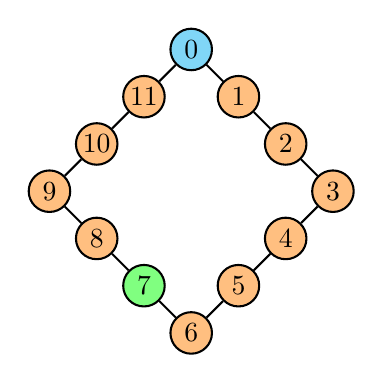
\begin{tikzpicture}[scale=0.6, every node/.style={circle, draw}]
			\tikzstyle{every node}=[circle, draw, fill=orange!50,
			inner sep=0pt, minimum width=15pt]
			
			
			\node[fill=cyan!50] (n0) at (0,3) {0};
			\node (n1) at (1,2) {1};
			\node (n2) at (2,1) {2};
			\node (n3) at (3,0) {3};
			\node (n4) at (2,-1) {4};
			\node (n5) at (1,-2) {5};
			\node (n6) at (0,-3) {6};
			
			\node (n11) at (-1,2) {11};
			\node (n10) at (-2,1) {10};
			\node (n9) at (-3,0) {9};
			\node (n8) at (-2,-1) {8};
			\node[fill=green!50] (n7) at (-1,-2) {7};
			
		
			\draw (n0) -- (n1);
			\draw (n1) -- (n2);
			\draw (n2) -- (n3);
			\draw (n3) -- (n4);
			\draw (n4) -- (n5);
			\draw (n5) -- (n6);
			\draw (n6) -- (n7);
			\draw (n7) -- (n8);
			\draw (n8) -- (n9);
			\draw (n9) -- (n10);
			\draw (n10) -- (n11);
			\draw (n11) -- (n0);
			
		\end{tikzpicture}
	\end{center}
	
	Define the event $B$ be $B = \set{T^+_0 > T_7}$. We are interested in finding $\prob_0(B)$. Now we can perform the first step argument as follows
	\[ p_0 = \frac{1}{2}(p_1 + p_{11}). \tag{3.1} \]
	Then we analyze each term in the right hand side of the equation above. For $p_1$ we have
	\[ \prob_1(B) = \underbrace{\prob_1(B|T_0>T_7)}_{1}\underbrace{\prob_1(T_0>T_7)}_{1/5} + \underbrace{\prob_1(B|T_0<T_7)}_{0}\underbrace{\prob_1(T_0<T_7)}_{6/7} = \frac{1}{5}. \]
	Note that $\prob_1(B|T_0>T_7)=1$ since it literally means the random walker reaches 7 before 0. Also $\prob_1(B|T_0<T_7)=0$ since the event $B$ is conditioned on reaching 0 before 7, which is clearly 0. The term $\prob_1(T_0>T_7)$ is computed using the Gambler's ruin analysis. Similarly, for the $p_{11}$ term we have
	\[ \prob_{11}(B) = \underbrace{\prob_{11}(B|T_0>T_7)}_{1}\underbrace{\prob_{11}(T_0>T_7)}_{1/7} + \underbrace{\prob_{11}(B|T_0<T_7)}_{0}\prob_{11}(T_0<T_7) = \frac{1}{7}. \]
	The rationale behind the values of the terms are the same as the ones discussed above. Now we can substitute everything in $(3.1)$
	\[ \boxed{p_0 = \frac{1}{2} (\frac{12}{35}) = \frac{6}{35}}. \]
	
\end{ans}
\begin{question}
	The Fibonacci sequence is the sequence $(F_n)_{n\geq0}$ defined by $F_0 = 0, F_1=1$ and 
	\[ F_{n+2} = F_{n+1} + F_n \quad \text{for } n\geq 0.  \]
	Find a general formula for $F_n$
\end{question}
\begin{ans}
	First, we construct the characteristic polynomial of the sequence. From the recursive formula we can write
	\[ X^2 = X + 1 \implies \boxed{X^2 - X - 1 = 0}. \]
	The roots of the equation is 
	\[ r_1, r_2 = \frac{1 \pm \sqrt{5}}{2}. \]
	Now the general formula will be
	\[ F_n = Ar_1^n + Br_2^n. \] 
	To find the coefficients, we utilize the first two terms 
	\[ 0 = A + B, \qquad 1 = \frac{1}{2}(A+B) + \frac{\sqrt{5}}{2}(A-B). \]
	This system of equations implies that
	\[ A = \frac{1}{\sqrt{5}}, \qquad B=\frac{-1}{\sqrt{5}}.  \]
	Thus the general formula will be
	\[ \boxed{F_n = \frac{1}{\sqrt{5}}((\frac{1+\sqrt{5}}{2})^n - \frac{1-\sqrt{5}}{2})^n)}. \]
	
	\qed
	
\end{ans}
\begin{question}
	Let $(X_n)$ be the simple random walk on the following graph. Compute $\prob_0(T_3<T_7)$.
	
	\begin{center}
		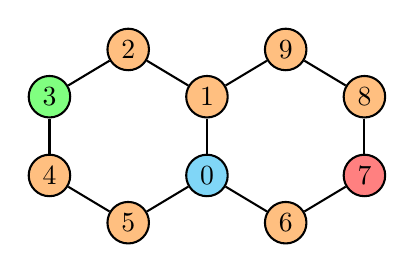
\begin{tikzpicture}[scale=1, every node/.style={circle, draw}]
			\tikzstyle{every node}=[circle, draw, fill=orange!50,
			inner sep=0pt, minimum width=15]
			
			
			\node[fill=cyan!50] (n0) at (0,0) {0};
			\node (n1) at (0,1) {1};
			\node (n2) at (-1,1.6) {2};
			\node[fill=green!50] (n3) at (-2,1) {3};
			\node (n4) at (-2,0) {4};
			\node (n5) at (-1,-0.6) {5};
			\node (n9) at (1,1.6) {9};
			\node (n8) at (2,1) {8};
			\node[fill=red!50] (n7) at (2,0) {7};
			\node (n6) at (1,-0.6) {6};

			\draw (n0) -- (n1);
			\draw (n1) -- (n2);
			\draw (n2) -- (n3);
			\draw (n3) -- (n4);
			\draw (n4) -- (n5);
			\draw (n5) -- (n0);
			\draw (n0) -- (n6);
			\draw (n6) -- (n7);
			\draw (n7) -- (n8);
			\draw (n8) -- (n9);
			\draw (n9) -- (n1);

			
		\end{tikzpicture}
	\end{center}
\end{question}
\begin{ans}
	For a much more simpler solution, let's define the two following notations
	\[ B = \{T_3 < T_7\}, \qquad p_v = \prob_v(B). \]
	Then, by first step argument at state $0$, we can write
	\[ p_0 = \frac{1}{3} (p_5 + p_6 + p_1).  \tag{5.1}\]
	Now we need to evaluate each of the terms in the right hand side. We start with $p_5$.
	\[ p_5 = \prob_5(B) = \underbrace{\prob_5(B|T_3<T_0)}_{1}\underbrace{\prob_5(T_3<T_0)}_{1/3} + \underbrace{\prob_5(B|T_3>T_0)}_{p_0}\underbrace{\prob_5(T_3>T_0)}_{2/3} = \frac{1}{3} + \frac{2}{3}p_0. \]
	note that $\prob_5(B|T_3<T_0) = 1$, since if we get to state 3, before getting to state 0, then it means that we have reached the state 3 before reaching the state 7, thus the event $B$ occurs with probability 1. Also $\prob_5(T_3<T_0) = 1/3$ from the Gambler's ruin. Furthermore $\prob_5(B|T_3>T_0) = p_0$ by using the Markov property, and finally $\prob_5(T_3>T_0) = 2/3$ by the Gambler's ruin. \\
	Now, we need to evaluate the term $p_6$. To analyze this term, we will do a first step argument starting at this point
	\[ p_6 = \prob_6(B) = \frac{1}{2}(\underbrace{p_7}_{0} + p_0) = \frac{p_0}{2}. \]
	Note that $p_7 = 0$, since then the event $B$ has not occurred. \\
	Finally, we need to analyze the term $p_1$. Again, by first step argument on this state we have
	\[ p_1 = \frac{1}{3}(p_0 + p_9 + p_2). \]	
	By doing a analysis on $p_9$ similar to the one we did for 5, we can write
	\[ p_9 = \prob_9(B)= \underbrace{\prob_9(B|T_7<T_1)}_{0}\prob_9(T_7<T_1) + \underbrace{\prob_9(B|T_7>T_1)}_{p_1}\underbrace{\prob_9(T_7>T_1)}_{2/3} = \frac{2}{3}p_1. \]
	The rationale behind the values for each term in the equation above, is exactly the same as in analyzing the terms of $p_5$.\\
	Now, we analyze the term $p_2$ by performing another first step analysis, similar to the one we did for state 6.
	\[ p_2 = \frac{1}{2}(\underbrace{p_3}_1 + p_1) = \frac{1}{2}(1+p_1). \]
	Now we can calculate $p_1$ in terms of $p_0$ which turns out to be
	\[ p_1 = \frac{6}{11}p_0 + \frac{3}{11}.  \]
	Now we insert all of the terms in the equation $(5.1)$ to get
	\begin{align*}
		&3p_0 = \frac{1}{3}+\frac{2}{3}p_0 + \frac{1}{2}p_0 + \frac{6}{11}p_0 + \frac{3}{11} \\ 
		&\implies 3p_0 - \frac{113}{66}p_0 = \frac{40}{33} \\
		&\implies p_0 = \frac{66}{85}\cdot\frac{40}{33} = \frac{16}{17}\\
		&\implies \boxed{p_0 = \frac{16}{17}}.
	\end{align*}


	\qed
	
	

\end{ans}

